\subsection{Problem}

\renewcommand{\theequation}{\theenumi}
\begin{enumerate}[label=\thesection.\arabic*.,ref=\thesection.\theenumi]
\numberwithin{equation}{enumi}
	\item Find the roots of the quadratic equation $6x^2-x-2=0$.
	The following python code computes roots of the quadratic equation represented in Fig.\ref{fig:qnineteen}.
	\begin{lstlisting}
	./codes/conics/q19.py
	\end{lstlisting}
	
	\solution For a general polynomial equation of degree 2,
	\begin{multline}
	p\brak{x,y} \implies Ax^2 +Bxy + Cy^2 +Dx + Ey + F = 0
	\\
	\text{The vector form is}
	\\
	\vec{x}^T\myvec{A&\frac{B}{2}\\\frac{B}{2}&C}\vec{x}  + \myvec{D&E}\vec{x} + F = 0 \label{eq:theend}
	\end{multline}
	Here \begin{align}y = 6x^2-x-2 \quad \text{The vector form is}
	\\
	\vec{x}^T\myvec{6&0\\0&0}\vec{x}  + \myvec{-1&-1}\vec{x} -2 = 0
	\end{align}
	Thus, from \ref{eq:theend}
	\begin{align}
	y = 0 \quad \implies 6x^2-x-2 = 0
	\\
	\brak{x+\frac{1}{2}}\brak{x-\frac{2}{3}} = 0
	\\
	x = \frac{-1}{2},\frac{2}{3}
	\end{align}
\begin{comment}
	Using the quadratic formula,
	\begin{equation}
		x = \frac{-(-1) \pm \sqrt{(-1)^2 - 4(6)(-2)}}{2(6)}
	\end{equation}
	which on solving we get the roots as -0.5 and 0.666
\end{comment}
	\begin{figure}[!ht]
	\centering
	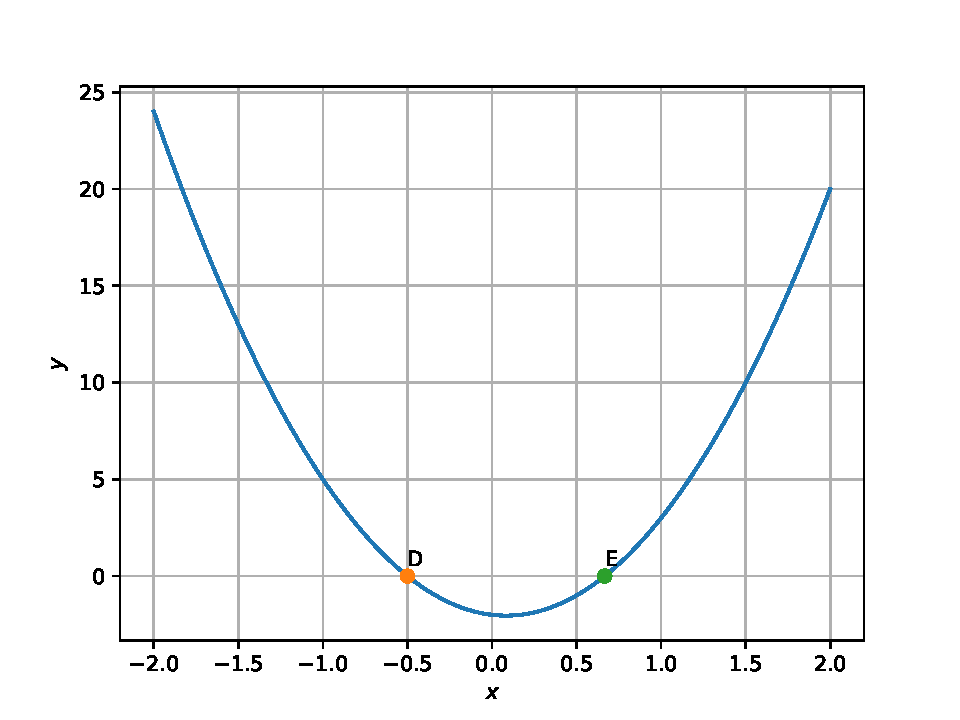
\includegraphics[width=\columnwidth]{./figs/conics/q19.pdf}
	\caption{Parabola of Q.5.1.5}
	\label{fig:qnineteen}	
	\end{figure}
	
	
\end{enumerate}
